\documentclass[a4paper]{article}

\title{Pok, Esame di Progettazione Applicazioni Web e Mobili}
\author{Filippo Biondi}
\date{Dicembre 2020}

\usepackage{graphicx}

\begin{document}

\maketitle

\renewcommand{\contentsname}{Contenuti}
\tableofcontents

\section{Introduzione}

Questa relazione analizza gli aspetti di implementazione dell'applicazione \textbf{Pok} realizzata per l'esame di \textbf{Progettazione Applicazioni Web e Mobili}

\section{Descrizione applicativo}

Pok è un'applicazione mobile che permette di creare \textbf{Post} anonimi legati alle coordinate geografiche dell'utente, i Post sono poi accessibili e commentabili anonimamente solo da utenti nei pressi delle coordinate in cui è stato creato il Post   

\section{Dettagli di Implementazione}

Questa sezione descrive i pattern e le tecnologie adottate per l'implementazione dell'applicativo

\newpage

\subsection{Frontend}

Il frontend di Pok è stato realizzato con l'sdk \textbf{Flutter}, utilizzando il pattern \textbf{BLoC} (\textbf{B}usiness \textbf{Lo}gic \textbf{C}omponent) che permette di gestire lo stato della UI attraverso dei componenti middleware 
chiamati BLoC che si pongono tra l' interfaccia utente e il codice per le chiamate all'API, essi comunicano i cambiamenti di stato alla UI attraverso uno \textbf{Stream} di eventi.

\subsubsection{Interfaccia utente}

L'interfaccia utente presenta 2 viste principali oltre a quella per l'autenticazione, una per la ricerca di post nelle vicinanze e una per la creazione di nuovi post

\vspace{1.05cm}

\begin{figure}[h!]
   \centering
   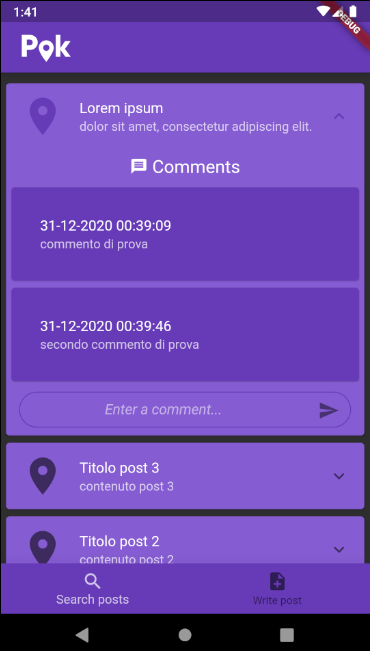
\includegraphics[scale=0.6]{ricercapost} 
   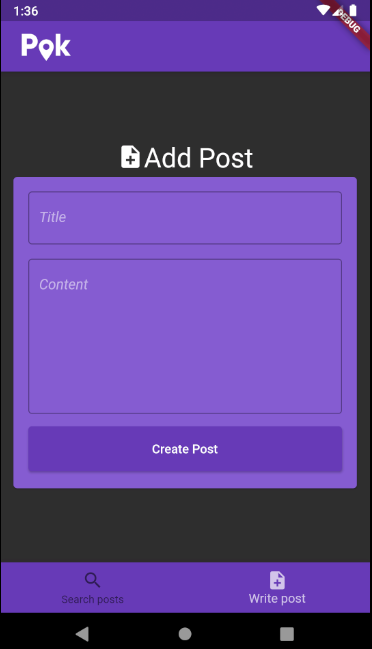
\includegraphics[scale=0.6]{aggiungipost} 
   \caption{(a) Ricerca post nelle vicinanze e commenti (b) Creazione nuovi post}
\end{figure}

\newpage

\subsection{Autenticazione}

L'autenticazione all'api è stata gestita utilizzando il servizio \textbf{Firebase}, con supporto all'autenticazione tramite account google.

\subsection{Backend}

Il server di backend è stato realizzato in \textbf{Rust} utilizzando il framework \textbf{Actix web} per la creazione della Rest API HTTP e la libreria \textbf{Diesel} per interfacciarsi al database \textbf{Postgresql}.
Non esistendo una release della libreria \textbf{Firebase Admin SDK} per il linguaggio Rust la verifica dei Token ID di Firebase per l'autenticazione è stata effettuata seguendo le linee guida di Google \cite{verificatoken} utilizzando
la libreria \textbf{jsonwebtoken} per la validazione di token jwt.

\subsection{Infrastruttura}

L'infrastruttura di Pok si compone di un server \textbf{VPS} che ospita una sottorete di container \textbf{Docker}, essa comprende un container per il server postgresql e un container per il server di backend, un proxy \textbf{NGINX} agisce da gateway e rende accessibile l'api del backend esternamente tramite \textbf{HTTPS}


\begin{figure}[h!]
   \centering
   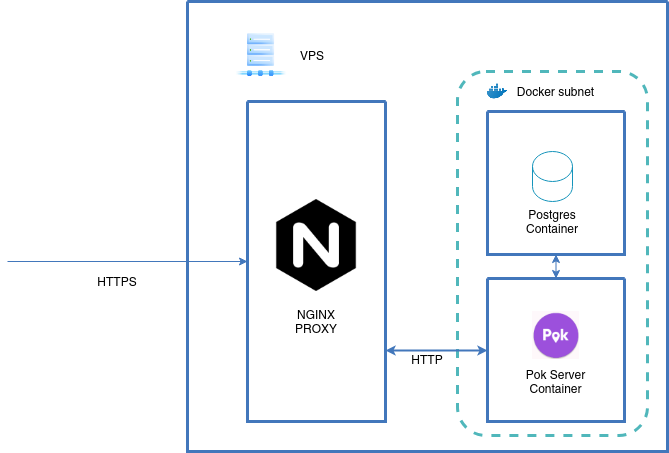
\includegraphics[scale=0.4]{infrastructure} 
   \caption{Rappresentazione grafica dell'infrastruttura di Pok}
\end{figure}

\begin{thebibliography}{9}

\bibitem{verificatoken}
Firebase: Verify ID Tokens
\\\texttt{https://firebase.google.com/docs/auth/admin/verify-id-tokens}

\end{thebibliography}

\end{document}
